
% ----------------------------------------------------------------------
%  Set the document class
% ----------------------------------------------------------------------
\documentclass[11pt,a4paper,twoside]{article}

% ----------------------------------------------------------------------
% Define external packages, language, margins, fonts and new commands
% ----------------------------------------------------------------------
%\input{preamble} 
\usepackage[utf8]{inputenc}   % <<<<< Linux
\usepackage[english]{babel} % <<<<< English
\usepackage{notoccite}
\usepackage[skip=0.5\baselineskip]{caption}
\hyphenation{GTKWave}
\usepackage{listings}
\usepackage[all]{nowidow}

%blind text
\usepackage{lipsum}

\usepackage{graphicx}
\graphicspath{ {./} {../../figlib/} }
\def\FontLn{% 16 pt normal
  \usefont{T1}{phv}{m}{n}\fontsize{16pt}{16pt}\selectfont}
\def\FontLb{% 16 pt bold
  \usefont{T1}{phv}{b}{n}\fontsize{16pt}{16pt}\selectfont}
\def\FontMn{% 14 pt normal
  \usefont{T1}{phv}{m}{n}\fontsize{14pt}{14pt}\selectfont}
\def\FontMb{% 14 pt bold
  \usefont{T1}{phv}{b}{n}\fontsize{14pt}{14pt}\selectfont}
\def\FontSn{% 12 pt normal
  \usefont{T1}{phv}{m}{n}\fontsize{12pt}{12pt}\selectfont}

% Use Arial font as default
%
\renewcommand{\rmdefault}{phv}
\renewcommand{\sfdefault}{phv}
\usepackage{geometry}	
\geometry{verbose,tmargin=2.5cm,bmargin=2.5cm,lmargin=2.5cm,rmargin=2.5cm}

%\usepackage{setspace}
%\renewcommand{\baselinestretch}{1.5}

\usepackage[pdftex]{hyperref} % enhance documents that are to be
                              % output as HTML and PDF
\hypersetup{colorlinks,       % color text of links and anchors,
                              % eliminates borders around links
%            linkcolor=red,    % color for normal internal links
            linkcolor=black,  % color for normal internal links
            anchorcolor=black,% color for anchor text
%            citecolor=green,  % color for bibliographical citations
            citecolor=black,  % color for bibliographical citations
%            filecolor=magenta,% color for URLs which open local files
            filecolor=black,  % color for URLs which open local files
%            menucolor=red,    % color for Acrobat menu items
            menucolor=black,  % color for Acrobat menu items
%            pagecolor=red,    % color for links to other pages
            pagecolor=black,  % color for links to other pages
%            urlcolor=cyan,    % color for linked URLs
            urlcolor=black,   % color for linked URLs
	          bookmarks=true,         % create PDF bookmarks
	          bookmarksopen=false,    % don't expand bookmarks
	          bookmarksnumbered=true, % number bookmarks
	          pdftitle={report},
            pdfauthor={Andre C. Marta},
%            pdfsubject={Thesis Title},
%            pdfkeywords={Thesis Keywords},
            pdfstartview=FitV,
            pdfdisplaydoctitle=true}

\usepackage[numbers,sort&compress]{natbib} % <<<<< References in numbered list [1],[2],...
\usepackage{subcaption} 
\usepackage{mdframed}

%%%%%%%%%%%%%%%%%%%%%%%%%%%%%%%%%%%%%%%%%%%%%%%%%%%%%%%%%%%%%%%%%%%%%%%%
%     Begin Document                                                   %
%%%%%%%%%%%%%%%%%%%%%%%%%%%%%%%%%%%%%%%%%%%%%%%%%%%%%%%%%%%%%%%%%%%%%%%%


\begin{document}

% Set plain page style (no headers, footer with centered page number)
\pagestyle{plain}

% Set roman numbering (i,ii,...) before the start of chapters
%\pagenumbering{roman}

% ----------------------------------------------------------------------
%  Cover page
% ----------------------------------------------------------------------
%%%%%%%%%%%%%%%%%%%%%%%%%%%%%%%%%%%%%%%%%%%%%%%%%%%%%%%%%%%%%%%%%%%%%%%%
%                                                                      %
%     File: Thesis_FrontCover.tex                                      %
%     Tex Master: Thesis.tex                                           %
%                                                                      %
%     Author: Andre C. Marta                                           %
%     Last modified :  2 Jul 2015                                      %
%                                                                      %
%%%%%%%%%%%%%%%%%%%%%%%%%%%%%%%%%%%%%%%%%%%%%%%%%%%%%%%%%%%%%%%%%%%%%%%%

\thispagestyle {empty}

% IST Logo - Signature A
% parameters: bb=llx lly urx ury (bounding box), width=h_length, height=v_length, angle=angle, scale=factor, clip=true/false, draft=true/false. 

\includegraphics[bb=9.5cm 11cm 0cm 0cm,scale=0.29]{IST_A_CMYK_POS}

\begin{center}
%
% Figure (Image or plot)
\vspace{1.0cm}
% height = 50 mm
%\includegraphics[height=50mm]{Figures/Airbus_A350.jpg}

% Title, author and degree
\vspace{1cm}
{\FontLb Circuit Theory and Electronics Fundamentals} \\ % <<<<< EDIT TITLE
\vspace{1cm}
{\FontSn Integrated Master in Aerospace Engineering, Técnico, University of Lisbon} \\ % <<<<< EDIT COURSE
\vspace{1cm}
{\FontSn João Pedro Carvalho, 95808} \\
\vspace{0.3cm}
{\FontSn Mafalda Santos, 95820} \\
\vspace{0.3cm}
{\FontSn Manuel Barbosa, 95824} \\
\vspace{1cm}
{\FontSn March 22, 2021} \\ % <<<<< EDIT DATE (corresponds to date of oral examination)
%
\end{center}





% ----------------------------------------------------------------------
% Dedication page (optional)
% ----------------------------------------------------------------------
%\input{dedication} 
%\cleardoublepage

% ----------------------------------------------------------------------
%  Acknowledgments (optional)
% ----------------------------------------------------------------------
%\input{acknowledgements}
%\cleardoublepage

% ----------------------------------------------------------------------
%  Abstract (both in English and Portuguese)
% ----------------------------------------------------------------------
%\input{resumo} 
%\cleardoublepage

%\input{abstract} 

% ----------------------------------------------------------------------
%  Table of contents, list of tables, list of figures and nomenclature
% ----------------------------------------------------------------------

% Table of contents
%
\tableofcontents

% List of tables
%\addcontentsline{toc}{section}{\listtablename}
%\listoftables
%\cleardoublepage 

% List of figures
%\addcontentsline{toc}{section}{\listfigurename}
%\listoffigures
%\cleardoublepage 

% Set arabic numbering (1,2,...) after preface
%
%\setcounter{page}{1}
%\pagenumbering{arabic}

% ----------------------------------------------------------------------
%  Body
% ----------------------------------------------------------------------

\pagebreak
\section{Introduction}
\label{sec:introduction}

% state the learning objective 
The objective of this laboratory assignment is to study a circuit containing one independent and one dependent voltage sources, $V_a$ and $V_c$ respectively, as well as one independent and one dependent current sources, $I_d$ and $I_b$, connected to 7 resistors. The circuit can be seen in Figure~\ref{fig:circuito_t1}.



In Section~\ref{sec:analysis}, a theoretical analysis of the circuit is
presented. In Section~\ref{sec:simulation}, the circuit is analysed by
simulation, and the results are compared to the theoretical results obtained in
Section~\ref{sec:analysis}. The conclusions of this study are outlined in
Section~\ref{sec:conclusion}.

\begin{figure}[H] \centering
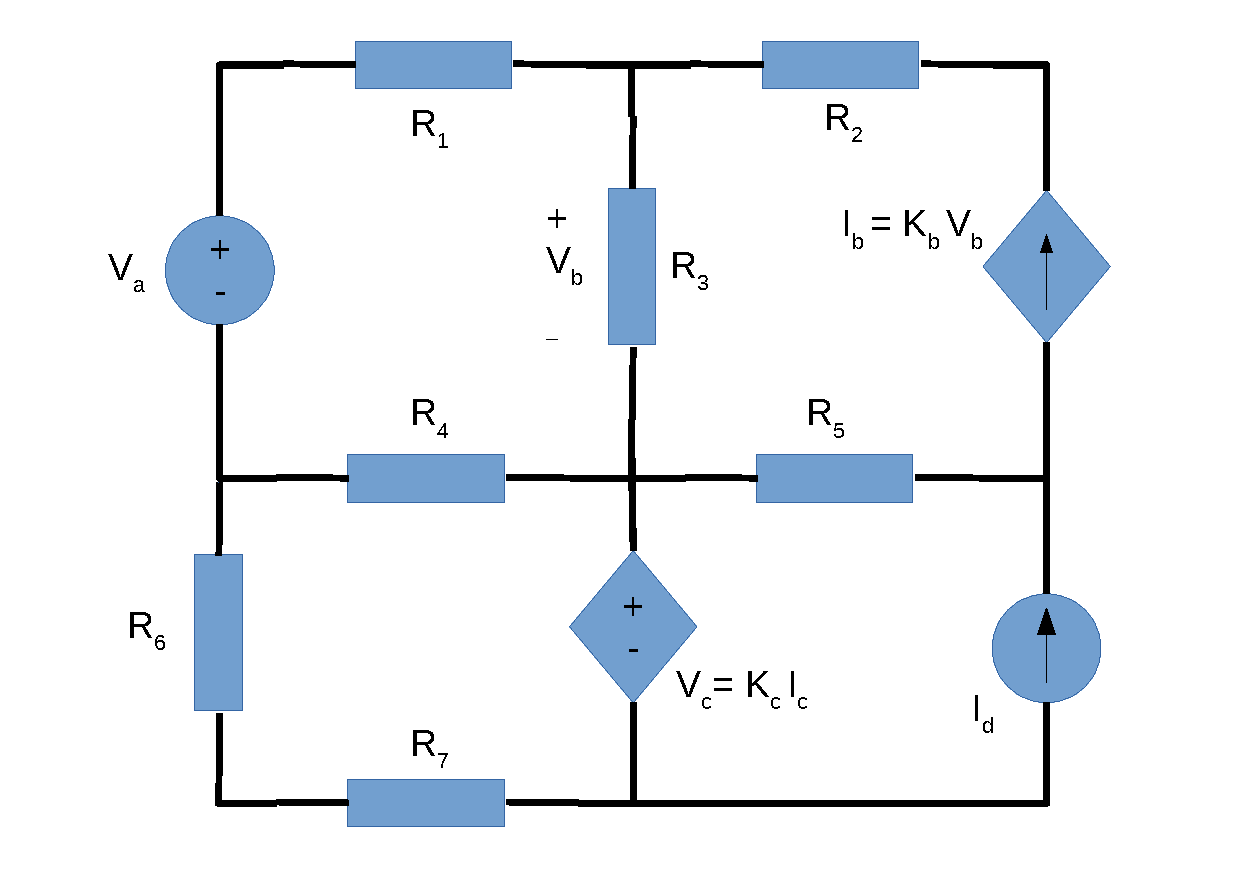
\includegraphics[width=0.5\linewidth]{circuito_T1.pdf}
\caption{Circuit for Lab T1.}
\label{fig:circuito_t1}
\end{figure}



\section{Theoretical Analysis}
\label{sec:analysis}

In this section, the circuit shown in Figure~\ref{fig:circuito_t2} is analysed
theoretically, mainly with Kirchoff's Current Law, initially for t<0, then the natural solution, forced and natural solution, and frequency response for t>0.

The circuit consists of 8 nodes. These were numbered from 1 to 8 as illustrated in Figure \ref{fig:circuito_t2}. Node 4 is the reference node, because it's connected to ground. The circuit contains 7 resistors, 1 capacitor, 1 independent source ($V_s$ for voltage source) and 2 dependent sources ($V_d$ for current controlled voltage source and $I_b$ for voltage controlled current source).


\subsection{RC circuit (t<0)}

For t<0, vs(t)=Vs.


Apllying Kirchoff's Current Law (KCL) to nodes 2, 3, 4, 6 and 7 we get four equations:

\begin{equation}
  (V_2-V_1)G_1+(V_2-V_3)G_2+(V_2-V_5)G_3=0.
  \label{eq:n2}
\end{equation}

\begin{equation}
  K_b(V_2-V_5)+(V_2-V_3)G_2=0.
  \label{eq:n3}
\end{equation}

\begin{equation}
  V_4=0.
  \label{eq:n4}
\end{equation}

\begin{equation}
  -I_c+(V_5-V_6)G_5-K_b(V_2-V_5)=0.
  \label{eq:n6}
\end{equation}

\begin{equation}
  (V_4-V_7)G_6+(V_8-V_7)G_7=0.
  \label{eq:n7}
\end{equation}

In addition, because voltage source $V_s$ is connected between the reference node and a non reference node, we simply set the voltage at the non-reference node equal to the voltage of the voltage source.

\begin{equation}
  V_1=V_s.
  \label{eq:n1}
\end{equation}

As the voltage source $V_d$ is between two non reference nodes then it forms a supernode whose analysis is done as following:

\begin{equation}
  (V_4-V_5)G_4+(V_2-V_5)G_3+(V_6-V_5)G_5+I_c+(V_7-V_8)G_7=0.
  \label{eq:superno}
\end{equation}

\begin{equation}
  (V_5-V_8)=K_c(V_4-V_7)G_6.
  \label{eq:Vd}
\end{equation}

Recognizing a steady state in our analysis of this RC circuit, we can also see that:

\begin{equation}
  I_c=0.
  \label{eq:Ic}
\end{equation}

The solution is obtained by solving Equations~(\ref{eq:n1}), ~(\ref{eq:n2}), ~(\ref{eq:n3}), ~(\ref{eq:n4}), ~(\ref{eq:superno}), ~(\ref{eq:Vd}), ~(\ref{eq:n6}) and ~(\ref{eq:n7}), which are shown in matrix form in the Appendix. The results are illustrated in Table~\ref{tab:tab1}.

\begin{table}[ht]
  \centering
  \begin{tabular}{ |c|c|}
 \hline
 {\bf Name} & {\bf Value[A or V]} \\
 \hline\hline
  $V_1$ & \partialinput{4}{4}{../mat/tab1.tex}\\
 \hline
 $V_2$ & \partialinput{9}{9}{../mat/tab1.tex} \\
 \hline
 $V_3$ & \partialinput{14}{14}{../mat/tab1.tex} \\
 \hline
 $V_4$ & \partialinput{19}{19}{../mat/tab1.tex} \\
 \hline
 $V_5$ & \partialinput{24}{24}{../mat/tab1.tex} \\
 \hline
 $V_6$ & \partialinput{29}{29}{../mat/tab1.tex} \\
\hline
 $V_7$ & \partialinput{34}{34}{../mat/tab1.tex} \\
 \hline
 $V_8$ & \partialinput{39}{39}{../mat/tab1.tex} \\
 \hline
 $@I_R1$ & \partialinput{44}{44}{../mat/tab1.tex} \\
 \hline
 $@I_R2$ & \partialinput{49}{49}{../mat/tab1.tex} \\
 \hline
 $@I_R3$ & \partialinput{54}{54}{../mat/tab1.tex} \\
 \hline
 $@I_R4$ & \partialinput{59}{59}{../mat/tab1.tex} \\
 \hline
 $@I_R5$ & \partialinput{64}{64}{../mat/tab1.tex} \\
 \hline
 $@I_R6$ & \partialinput{69}{69}{../mat/tab1.tex} \\
 \hline
 $@I_R7$ & \partialinput{74}{74}{../mat/tab1.tex} \\
 \hline
 $@I_b$ & \partialinput{79}{79}{../mat/tab1.tex} \\
 \hline
 $@I_c$ & \partialinput{84}{84}{../mat/tab1.tex} \\
 \hline
 $@I_d$ & \partialinput{89}{89}{../mat/tab1.tex} \\
 \hline
\end{tabular}
  \caption{Nodal voltages and branch currents for t<0. A variable preceded by @ is of type {\em current}
    and expressed in Ampere; other variables are of type {\it voltage} and expressed in Volt.}
  \label{tab:tab1}
\end{table}

\subsection{Determining $R_eq$}

To determine the Natural Solution of $V_6$(t) for t>0, we must obtain the value of the equivalent resistance as seen from the capacitor. This is due to the time constant being $R_eq$C, thus explaining the need for this step.

To obtain this value, we "turn off" the independent sources in the circuit, and replace the capacitor with a voltage source $V_x$, whose value is $V_6$-$V_8$, $V_6$ and $V_8$ being the voltages obtained for t<0. Recognizing this continuity in the circuit, we use these as "inital conditions" to find the solution of $R_eq$.

First we replace Vs with a short circuit (Vs=0V) and replace equation ~(\ref{eq:n6}) with the new equation for node 6:

\begin{equation}
  V_6-V_8=V_x.
  \label{eq:V_x}
\end{equation}

Then we replace equation ~(\ref{eq:superno}) with a new supernode:

\begin{equation}
  (V_3-V_4)G_4+(V_6-V_7)G_7+(V_2-V_5)G_3-I_b=0.
  \label{eq:superno2}
\end{equation}

$R_eq$ will be the result of $V_x$/$I_x$, $I_x$=-$I_c$.

The solution is obtained by solving Equations~(\ref{eq:n1}), ~(\ref{eq:n2}), ~(\ref{eq:n3}), ~(\ref{eq:n4}), ~(\ref{eq:superno2}), ~(\ref{eq:Vd}), ~(\ref{eq:V_x}) and ~(\ref{eq:n7}), and is illustrated in Table~\ref{tab:tab2}.

\begin{table}[h]
  \centering
  \begin{tabular}{ |c|c|}
 \hline
 {\bf Name} & {\bf Value[A or V or Ohm]} \\
 \hline
 $V_1$ & \partialinput{4}{4}{../mat/tab2.tex}\\
 \hline
 $V_2$ & \partialinput{9}{9}{../mat/tab2.tex} \\
 \hline
 $V_3$ & \partialinput{14}{14}{../mat/tab2.tex} \\
 \hline
 $V_4$ & \partialinput{19}{19}{../mat/tab2.tex} \\
 \hline
 $V_5$ & \partialinput{24}{24}{../mat/tab2.tex} \\
 \hline
 $V_6$ & \partialinput{29}{29}{../mat/tab2.tex} \\
\hline
 $V_7$ & \partialinput{34}{34}{../mat/tab2.tex} \\
 \hline
 $V_8$ & \partialinput{39}{39}{../mat/tab2.tex} \\
 \hline
 $@I_R1$ & \partialinput{44}{44}{../mat/tab2.tex} \\
 \hline
 $@I_R2$ & \partialinput{49}{49}{../mat/tab2.tex} \\
 \hline
 $@I_R3$ & \partialinput{54}{54}{../mat/tab2.tex} \\
 \hline
 $@I_R4$ & \partialinput{59}{59}{../mat/tab2.tex} \\
 \hline
 $@I_R5$ & \partialinput{64}{64}{../mat/tab2.tex} \\
 \hline
 $@I_R6$ & \partialinput{69}{69}{../mat/tab2.tex} \\
 \hline
 $@I_R7$ & \partialinput{74}{74}{../mat/tab2.tex} \\
 \hline
 $@I_b$ & \partialinput{79}{79}{../mat/tab2.tex} \\
 \hline
 $@I_c$ & \partialinput{84}{84}{../mat/tab2.tex} \\
 \hline
 $@I_d$ & \partialinput{89}{89}{../mat/tab2.tex} \\
 \hline
 $*R_eq$ & \partialinput{89}{89}{../mat/tab2.tex} \\
 \hline
\end{tabular}
  \caption{Nodal Method. A variable preceded by @ is of type {\em current}
    and expressed in Ampere and one preceded by * is of type {\em resistance} and is expressed in Ohm; other variables are of type {\it voltage} and expressed in Volt.}
  \label{tab:tab2}
\end{table}


\subsection{Determining $V_6$(t)}

Now that we have $R_eq$, we can plot the natural solution as:

\begin{equation}
  V_6(t)=Vx*exp(-t/R_eq*C).
  \label{eq:natsol}
\end{equation}

This result is shown in figure \ref{fig:solnat}:

\begin{figure}[h] \centering
\includegraphics[width=0.5\linewidth]{solnat.eps}
\caption{Natural Solution of $V_6(t)$ for t>=0.}
\label{fig:solnat}
\end{figure}

\pagebreak
\subsection{Determining the Forced Solution for $V_6$(t)}
\label{sec:passo4}

To obtain the phasor voltage of $V_6$ ($PV_6$), we replace $V_s$ with its complex amplitude 1, and replace the capacitor with its Impedance $Z_c$=1/(jwC).

First we obtain the equation for $I_c$:

\begin{equation}
  I_c=(V_6-V_8)/Z_c.
  \label{eq:icimpe}
\end{equation}

For the supernode, we use the following equation:

\begin{equation}
  (V_1-V_2)G_1+(V_4-V_5)G_4+I_d=0.
  \label{eq:supernopasso4}
\end{equation}

The solution is obtained by solving Equations~(\ref{eq:n1}), ~(\ref{eq:n2}), ~(\ref{eq:n3}), ~(\ref{eq:n4}), ~(\ref{eq:supernopasso4}), ~(\ref{eq:Vd}), ~(\ref{eq:n6}) and ~(\ref{eq:n7}), and is illustrated in Table~\ref{tab:tab3}.

\begin{table}[h]
  \centering
  \begin{tabular}{ |c|c|}
 \hline
 {\bf Name} & {\bf Value[V]} \\
 \hline
 $PV_1$ & \partialinput{4}{4}{../mat/tab3.tex}\\
 \hline
 $PV_2$ & \partialinput{9}{9}{../mat/tab3.tex} \\
 \hline
 $PV_3$ & \partialinput{14}{14}{../mat/tab3.tex} \\
 \hline
 $PV_4$ & \partialinput{19}{19}{../mat/tab3.tex} \\
 \hline
 $PV_5$ & \partialinput{24}{24}{../mat/tab3.tex} \\
 \hline
 $PV_6$ & \partialinput{29}{29}{../mat/tab3.tex} \\
\hline
 $PV_7$ & \partialinput{34}{34}{../mat/tab3.tex} \\
 \hline
 $PV_8$ & \partialinput{39}{39}{../mat/tab3.tex} \\
 \hline
\end{tabular}
  \caption{Phasor voltages. Variables are of type {\it voltage} and expressed in Volt.}
  \label{tab:tab3}
\end{table}


\subsection{Determining the total solution}

Now we finally have the solution for $V_6$(t) (t>0), with the following expression:

\begin{equation}
  V_6(t)=Vx*exp(-t/R_eq*C)+PV_6*sin(wt).
  \label{eq:totalsol}
\end{equation}

Because in subsection 2.1 we calculated the values for t<0, we can plot the final solution, as shown in figure \ref{fig:soltotal}:

\begin{figure}[h] \centering
\includegraphics[width=0.5\linewidth]{soltotal.eps}
\caption{Final solution of $V_6(t)$ (orange) and $V_s(t)$ (blue).}
\label{fig:soltotal}
\end{figure}


\subsection{Frequency Response}

To analize the frequency response, we used the same system of equations as found in subsection ~(\ref{sec:passo4}), calculating $PV_6$,$PV_s$ and $PV_6$-$PV_8$ ($PV_c$) for different frequencies. For each result of these complex vectors, the absolute value and the angle was saved. 

The absolute values are shown in figure \ref{fig:mag}, in dB, representing the magnitude response, with the frequencies in a logarithmic scale.

\begin{figure}[h] \centering
\includegraphics[width=0.5\linewidth]{mag.eps}
\caption{Magnitude response of $V_6(t)$ (red), $V_c(t)$ (blue) and $V_s(t)$ (green)}
\label{fig:mag}
\end{figure}

The magnitude of $V_s(t)$ doesn't change with the frequency of the signal and therefore it's always 1 (0 in dB). However, the magnitude of $V_6$ changes with the frequency, firstly reducing and then staying constant. The magnitude of $V_c(t)$, which is a low pass filter, changes accordingly to what is expected of an RC circuit, with the increase of the frequency reducing the module of impedance and magnitude ($Z_c$=1/jwC).

Because the phase of the Voltage Signal $V_s$ is 0, the phase of each voltage, for each frequency, is just the angles saved, in degrees. The plot for these is also shown in figure \ref{fig:phase}, with the frequencies also in a logarithmic scale.

\begin{figure}[h] \centering
\includegraphics[width=0.5\linewidth]{phase.eps}
\caption{Phase response of $V_6(t)$ (red) and $V_c(t)$ (blue).}
\label{fig:phase}
\end{figure}



























\section{Simulation Analysis}
\label{sec:simulation}

\subsection{Envelope detector}
The simulated results of the envelope detector output are compared to the theoretical results as shown below in Figures \ref{fig:sim_env} and \ref{fig:theo_env}, respectively.


\begin{figure} [ht]
\centering
\begin{minipage}{.5\textwidth}
  \centering
  \includegraphics[width=0.9\linewidth]{../sim/transv2.pdf}
  \captionof{figure}{Simulated Envelope detector voltage output}
  \label{fig:sim_env}
\end{minipage}%
\begin{minipage}{.5\textwidth}
  \centering
  \includegraphics[width=0.9\linewidth]{venvlope.eps}
  \captionof{figure}{Theoritical Envelope detector voltage output}
  \label{fig:theo_env}
\end{minipage}
\end{figure}

The theoretical ripple in the envelope detector is considerably smaller than the simulated one, due to the approximations made in the theoretical diode model.




\pagebreak
\subsection{Output Voltage}
The simulated results of the voltage output are compared to the theoretical results as shown below in Figures \ref{fig:sim_vout} and \ref{fig:theo_vout}, respectively.

\begin{figure} [h]
\centering
\begin{minipage}{.5\textwidth}
  \centering
  \includegraphics[width=0.9\linewidth]{../sim/transv4.pdf}
  \captionof{figure}{Simulated voltage output.}
  \label{fig:sim_vout}
\end{minipage}%
\begin{minipage}{.5\textwidth}
  \centering
  \includegraphics[width=0.9\linewidth]{vout.eps}
  \captionof{figure}{Theoritical voltage output.}
  \label{fig:theo_vout}
\end{minipage}
\end{figure}

Once again, the theoretical ripple is considerably smaller than the simulated one, due to the approximations made in the theoretical diode model.

It is also notable that the output voltage values are always higher than both 12V and the simulation's values, which vary between higher and lower than 12V.  

\pagebreak
The voltage output errors ($V_{out}$ - 12) of the simulation and the theoretical analysis are shown above in Figures \ref{fig:sim_error} and \ref{fig:theo_error}, respectively.


\begin{figure}
\centering
\begin{minipage}{.5\textwidth}
  \centering
  \includegraphics[width=0.8\linewidth]{../sim/trans1.pdf}
  \captionof{figure}{Simulated voltage output error.}
  \label{fig:sim_error}
\end{minipage}%
\begin{minipage}{.5\textwidth}
  \centering
  \includegraphics[width=0.8\linewidth]{erro.eps}
  \captionof{figure}{Theoritical voltage output error.}
  \label{fig:theo_error}
\end{minipage}
\end{figure}

The output voltage error is always positive and higher than the simulation's, which varies between positive and negative.


Comparing the Voltage ripple and VDC of the simulated and theoretical analysis in tables \ref{tab:sim} and \ref{tab:tab1}, respectively:

\begin{table}[h]
  \centering
  \begin{tabular}{|l|r|}
    \hline    
    {\bf Name} & {\bf Value [V]} \\ \hline
    \input{../sim/passo2}
  \end{tabular}
  \caption{Simulated results. mean(v(4)) is the average outuput voltage and vecmax(v(4))-vecmin(v(4)) is the maximum value of ripple. The last value is the merit of the circuit.}
  
  \label{tab:sim}
\end{table}

\begin{table}[h]
  \centering
  \begin{tabular}{ |c|c|}
 \hline
 {\bf Name} & {\bf Value[V]} \\
 \hline\hline
  $V_{DC}$ & \partialinput{4}{4}{../mat/tab1.tex}\\
 \hline
 $V_{ripple}$ & \partialinput{9}{9}{../mat/tab1.tex} \\
 \hline
 \end{tabular}
  \caption{Theoretical values. $V_{DC}$ is the average outuput voltage.}
  \label{tab:tab1}
\end{table}

The relative error for the average output voltage is aproximately 0.713\%.
The relative error for the maximum ripple is aproximately -34.22\%. These errors are once again due to the approximations made in the theoretical diode model.

The merit value is 3.754540e-01.

\pagebreak
\section{Conclusion}
\label{sec:conclusion}

We have successfully analysed theoretically the given circuit using the Octave maths tool to calculate the transient and frequency response. By comparing with the results obtained with the simulation done with the Ngspice tool, we could see they were mostly  identical with relative errors of the ordem of magnitude 10 to the power of -5, which allowed us to confirm the validity of the methods and their precision in simple circuits like the one given.
 
\pagebreak
\section{Appendix}
\begin{equation}
\begin{pmatrix}
    -G1 & G1+G2+G3 & -G2 & 0 & -G3 & 0 & 0 & 0 \\
    0 & Kb+G2 & -G2 & 0 & -Kb & 0 & 0 & 0 \\
    0 & 0 & 0 & 1 & 0 & 0 & 0 & 0 \\
    0 & -Kb & 0 & 0 & G5+Kb & -G5 & 0 & 0 \\
    0 & 0 & 0 & G6 & 0 & 0 & -G6-G7 & G7 \\
    1 & 0 & 0 & 0 & 0 & 0 & 0 & 0 \\
    0 & G3 & 0 & G4 & -G4-G3-G5 & G5 & G7 & -G7 \\
    0 & 0 & 0 & -KcG6 & 1 & 0 & KcG6 & -1\\
    
\end{pmatrix}
\end{equation}

\begin{equation}
\begin{pmatrix}
  V1 \\
  V2 \\
  V3 \\
  V4 \\
  V5 \\
  V6 \\
  V7 \\
  V8 \\
 
\end{pmatrix}
\end{equation}

\begin{equation}
\begin{pmatrix} 
  0 \\
  0 \\
  0 \\
  0 \\
  0 \\
  Vs \\
  0 \\
  0 \\
\end{pmatrix}
\end{equation}


%\cleardoublepage

% ----------------------------------------------------------------------
%  Bibliography
% ----------------------------------------------------------------------
%\addcontentsline{toc}{section}{\bibname}
%\bibliographystyle{abbrvunsrtnat} % <<<<< SELECT IF USING REFERENCES BY NUMBER (CITATION ORDER)
%\bibliography{../../../BIBfile.bib}

% ----------------------------------------------------------------------
\end{document}
% ----------------------------------------------------------------------

